% Source transcribed from thesis Figure A.10 (physical PDF p. 135).
% The screenshot contains the complete document, which is preserved here.
% It is independent of the freshly generated fixtures in this directory.
\documentclass{article}
\usepackage{tikz}
\usetikzlibrary{automata,positioning,arrows}
\pagestyle{empty}
\begin{document}
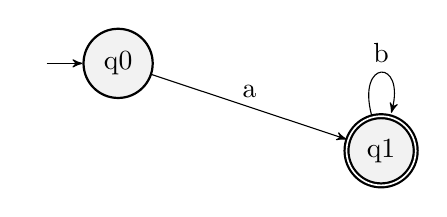
\begin{tikzpicture}[
  ->,
  >=stealth',
  node distance=3cm,
  every state/.style={thick, fill=gray!10},
  initial text=$ $,
]
\node[state, initial] (q0) at (-2.56, 0.89) {q0};
\node[state, accepting] (q1) at (0.78, -0.22) {q1};
\draw
  (q0) edge[above] node{a} (q1)
  (q1) edge[loop above] node{b} (q1);
\end{tikzpicture}
\end{document}
